% This file was converted to LaTeX by Writer2LaTeX ver. 0.5
% see http://www.hj-gym.dk/~hj/writer2latex for more info
\documentclass{article}
\usepackage[ascii]{inputenc}
\usepackage[T1]{fontenc}
\usepackage[english]{babel}
\usepackage{amsmath,amssymb,amsfonts,textcomp}
\usepackage{color}
\usepackage{array}
\usepackage{hhline}
\usepackage{hyperref}
\hypersetup{pdftex, colorlinks=true, linkcolor=blue, citecolor=blue, filecolor=blue, pagecolor=blue, urlcolor=blue, pdftitle=, pdfauthor=qiangwz, pdfsubject=, pdfkeywords=}
\usepackage[pdftex]{graphicx}
% List styles
\newcommand\liststyleLi{%
\renewcommand\theenumi{\arabic{enumi}}
\renewcommand\theenumii{\arabic{enumii}}
\renewcommand\theenumiii{\arabic{enumiii}}
\renewcommand\theenumiv{\arabic{enumiv}}
\renewcommand\labelenumi{\theenumi.}
\renewcommand\labelenumii{\theenumii.}
\renewcommand\labelenumiii{\theenumiii.}
\renewcommand\labelenumiv{\theenumiv.}
}
\newcommand\liststyleLii{%
\renewcommand\labelitemi{${\bullet}$}
\renewcommand\labelitemii{${\circ}$}
\renewcommand\labelitemiii{${\blacksquare}$}
\renewcommand\labelitemiv{${\bullet}$}
}
\newcommand\liststyleLiii{%
\renewcommand\labelitemi{${\bullet}$}
\renewcommand\labelitemii{${\circ}$}
\renewcommand\labelitemiii{${\blacksquare}$}
\renewcommand\labelitemiv{${\bullet}$}
}
\newcommand\liststyleLv{%
\renewcommand\theenumi{\arabic{enumi}}
\renewcommand\theenumii{\arabic{enumii}}
\renewcommand\theenumiii{\arabic{enumiii}}
\renewcommand\theenumiv{\arabic{enumiv}}
\renewcommand\labelenumi{\theenumi.}
\renewcommand\labelenumii{\theenumii.}
\renewcommand\labelenumiii{\theenumiii.}
\renewcommand\labelenumiv{\theenumiv.}
}
% Page layout (geometry)
\setlength\paperwidth{8.5in}
\setlength\paperheight{11in}
\setlength\voffset{-1in}
\setlength\hoffset{-1in}
\setlength\topmargin{0.7874in}
\setlength\oddsidemargin{0.7874in}
\setlength\textheight{9.4251995in}
\setlength\textwidth{6.9251995in}
\setlength\footskip{0.0cm}
\setlength\headheight{0cm}
\setlength\headsep{0cm}
% Footnote rule
\setlength{\skip\footins}{0.0469in}
\renewcommand\footnoterule{\vspace*{-0.0071in}\setlength\leftskip{0pt}\setlength\rightskip{0pt plus 1fil}\noindent\textcolor{black}{\rule{0.25\columnwidth}{0.0071in}}\vspace*{0.0398in}}
% Pages styles
\makeatletter
\newcommand\ps@Standard{
  \renewcommand\@oddhead{}
  \renewcommand\@evenhead{}
  \renewcommand\@oddfoot{}
  \renewcommand\@evenfoot{}
  \renewcommand\thepage{\arabic{page}}
}
\makeatother
\pagestyle{Standard}
\title{}
\begin{document}
{\centering
Towards cross-domain authentication and standardized attribute-based
authorization for ARC grid middleware
\par}


\bigskip

{\centering
Abstract
\par}

\ In order to make the access to Grids as simple as possible, security
including authentication and authorization is one of the most important
challenges in production Grids, especially when the Grid applications
are across multiple administration domains as well as across
heterogeneous Grid middlewares, such as some widely scaled eScience
applications which needs to coordinate resources sharing among
collection of autonomous institutions with different Grid middlewares
running on these resources. In this paper, we describe the security
implementation and consideration in new version of Advanced Resource
Connector (ARC) middleware, where the above issues have been exploited.
The main goal of ARC implementation in terms of security is to let the
middleware be capable to \ interoperate with other Grid middlewares by
leveraging standard specifications. The key aspect of the work we have
done is to enhance the current proxy certificate based delegation and
authentication by utilizing the Security Assertion Markup Languages
(\textit{SAML}) single sign-on (SSO) profile, WS-Security in order to
achieve cross-domain authentication, as well as to enhance the
Attribute Certificate (AC) based authorization by utilizing the SAML
\ attribute query profile in order to achieve standardized
attribute-based authorization. \ 


\bigskip

\liststyleLi
\begin{enumerate}
\item[] {\centering
1. Introduction
\par}
\end{enumerate}
Grids provides the technology for large scaled, cross domains
collaboration where the users work on resources and sharing data which
are distributed across domains. This kind of collaboration is called
virtual organization (VO)[ref1]. The resources that contribute to the
VO could come from independent administrative domains, and even require
different security approaches for control the access to themselves. The
same heterogeneous situation even critically applies to users who need
to access the VO, because users holding one kind of credential could
need to travel through multiple resources with different security
approaches. To solve the above issues, the Grid middleware should
provide the following ability: The user which participates the VO
should be able to access data and resources without being required to
constantly do authentication at each resource or data; The VO should be
able to easily manage the privileges or memberships to the users, and
VO together with its resources should be able to easily manage the
authorization, given the condition that the resources are actually
owned by different administrative domains.

In grid community, Grid Security Infrastructure (GSI)[ref2] is the
\textit{de facto} standard about authentication and \ transport level
communication, which is builds on Public Key Infrastructure (PKI), an
architecture based on X.509 public key certificate. GSI implements some
enhancement (such as certificate delegation) based on standard SSL/TLS
protocol. Mutual authentication is required by GSI, and is the default
configuration for GSI based grid deployment; and X.509 certificates is
required for both of the client and service sides in order to achieve
mutual authentication. X.509 certificates is issued by trusted third
party called certificate authorities (CA), and then CAs constitute
trust federation and guarantee two different X.509 certificates from
different CAs can accomplish authentication to each other. So if a user
would access grid system, he/she should own a X.509 certificate which
is issued by a CA that is trusted by other{\textquotesingle}s entity in
the GSI based grid system.

In terms of the virtual organization issues mentioned earlier, GSI and
some other related solutions like virtual organization management
service (VOMS) [ref3] has partly solved the them in some sense. The
identity delegation and X.509 proxy certificate initiated by GSI can
achieve single sign-on, so that the need to re-enter the
user{\textquotesingle}s pass phrase for authentication can be avoided
by creating the proxy certificate, even if some local or remote
entities access access resources on behalf of this user. \ As the most
successful grid authorization model, VOMS adopts X.509 Attribute
Certificate[ref4]. Attribute certificate is signed by VOMS server and
then binded to proxy certificates by client, \ and attributes
certificate includes the VO memberships which is associated with the
proxy certificate{\textquotesingle}s identity. Essentially the
resources can make access control decision based on parsing the VO
membership attributes from the homogeneous attribute certificate. 

\ \ \ \ The VO is essentially supposed to be able to provide resource
sharing capability with resources running under heterogeneous
systems/middlewares. This goal can be achieved using Web Service
Architecture (WSA). Therefore, the Web Service technology has been
converged into Grid computing middlewares. The Web Service technology
has been adopted by Globus toolkit, gLite, as well as the ARC.
Actually, utilizing Web Service technology and providing seamless
interoperability with other middlewares is one of the main goals of the
new version of ARC middleware.

Unfortunately, the existing grid security solutions such as GSI and VOMS
do not apply to Web Service \ based application very well due to the
following reasons:

\liststyleLii
\begin{itemize}
\item Firstly, the common implementation for Web Service does not
necessarily recognize and then properly verify and parse the
certificate, since comparing with usual X.509 certificate, proxy
certificate needs different treatment such as proxy path verification. 
\item Secondly, the X.509 Attribute Certificate has not been adopted by
any Web Service implementation at all. 
\item Thirdly, what is even worse is that the GSS API based confidential
communication has also not been adopted by Web Service implementation.
\item Finally, identity delegation is a good solution for user or
user{\textquotesingle}s representative (on behalf of the user) to
move/travel from one resource to another resource. But since the
identity delegation has been completely coupled with the GSI
confidential communication process, it is not possible for the existing
identity delegation solution to be used by Web Service applications.
\end{itemize}
There is some effort to add GSI support to adapt to the strict security
requirement including GSI from grid middlewares, such as GSI plug-in
for gSOAP[ref6]. However, this kind of solution
doesn{\textquotesingle}t help the existing grid middlewares
interoperate with other common Web Service implementation. Instead, Web
Service implementations commonly use the WS-Security, Security
Assertion Markup Languages (SAML), and standard SSL/TLS as well as
standard X.509 certificate when considering security. \ 

\ \ \ \ Moreover, the current grid security solutions require each user
to possess a X.509 certificate. But the process to get a certificate
may take quite long time, since the requester needs to be checked and
approved by the Registration Authority (RA) and then the Certificate
Authority (CA) can issue the certificate according to the approval from
RA. Meanwhile the process to use the certificate is also not so easy
for the wider less-IT focused research community to deal with, since
the user need to generate the proxy certificate by using the grid
specific command lines, such as \textit{grid-proxy-init}, and
\textit{voms-proxy-init}. On the other hand, users could most normally
have some local community/institutional credentials such as
username/passwords to which users are more familiar. To enable users
use their own community credential instead of the X.509 certificate to
access grid is a promising solution to make the grid be more easily
accessible. 

\ \ \ \ The above analysis shows that in order to achieve
interoperability and accessibility for user to access grid system, we
need to address the mismatch between the different security solutions
from different middlewares while keeping the changes as minimum as
possible and the benefits as much as possible; also need to address the
mismatch between user{\textquotesingle}s normal experience and
middleware requirement in order to ensure the access as simple as
possible.

\ \ The approach in the new version of ARC is to utilize the existing
Web Service standards, such as SAML and WS-Security, to achieve the
interoperability and accessibility without breaking existing grid
specific security protocols.

\ The rest of this paper is organized as follows: Section 2 shows the
ARC grid middleware, especially the architecture if the new version of
ARC. Section 3 describes the solution about cross-domain authentication
and single sign-on is presented, including a few solutions implemented
for bridging the mismatch in terms of authentication. \ Section 4
describes the implementation about standardized attribute querying for
authorization. Section 5 discusses the related research, and Section 6
concludes.


\bigskip


\bigskip


\bigskip

Based on OASIS WS-Trust 1.3 standard


\bigskip


\bigskip

Allows us to bridge security domains in a scalable manner

Allows the use of multiple token formats

pick which is best/supported for your product

Privacy can be protected across applications because:

\ Each application can get a different, opaque, ID

\ Each application receives only the attributes it needs

\ \ \ \ Attributes may be retrieved from places like VOMS, GUMS, etc.

\ \ \ \ When one application requests a token for use with another that
token \ may be encrypted so that only the receiving app may view its
data 

The STS serves as a point where policy decisions, such as \ whether App1
can talk to App2, can be made.

Removes the need for proprietary token related protocols

\ \ Supports a superset of current operations and works for more than
\ one token format


\bigskip


\bigskip

While we started our work on the STS in the grid space it \ became clear
it had other uses:

\ \ A portal wants to connect to a SOAP service to get information
\ about you but needs a SAML assertion to do it

\ \ A user wants to connect to an AFS server in a different domain
\ using the credentials from their domain

\ \ A user has a SAML assertion but needs a Kerberos ticket to
\ communicate with SharePoint

There are a number of token formats out there. \ Chances \ are high,
amongst all the software you have, more than one \ format is supported.

How will you prepare for the next greatest format to hit the \ street?


\bigskip


\bigskip


\bigskip


\bigskip

In ARC1, besides that GSI is supported for talking with external grid
services which are based on GSI, the standard TLS/SSL is also
supported.


\bigskip

{\centering
2. ARC grid middleware 
\par}

ARC(Advanced Resource Connector) is an open source grid middleware
solution released under GPL licence. ARC middleware initially aimed at
developing a grid middleware which provides characteristics such as
self-organized, fault-tolerant, non-intrusive, easy-management [fgcs
ARC paper]. \ Now \ the classic version of ARC provides grid services
such as grid job submission and management, resource characterization,
resource aggregation and discovery, basic data management, integration
of grid security solution, etc. Classic ARC has been deployed and used
in production environment, and been one of the mainly deployed grid
middlewares in Europe.

The new generation of ARC is funded by KnowARC project, and based on the
functionality and capabilities of the classic ARC middleware, it aims
at implementing a service-oriented middleware which will provide higher
levels of resource and user abstracting through well-defined web
service interface [Design document] in order to provide
interoperability with other service-based grid middlewares, as well as
other Web Service compatible applications.

As the key part of the implementation of new ARC middleware, there is a
lightweight web service container called HED (Hosting Environment
Daemon) which provides a host place for various services in application
level, as well as a host place for a bunch of components to support
flexible, interoperatible, and efficient communication mechanism. The
whole design of the HED is built around the idea of flexibility and
modularity, which means for the developer, he can easily concentrate on
the application level Web Service implementation by only using the core
minimum amount of components if he only would do application level
development, or he can easily concentrate on the middleware level
implementation such as supporting another communication protocol or
implementing authentication mechanism by using the core minimum amount
of components and external dependencies; also for the deployer, he can
easily configure and deploy the middleware and application for
different kinds of requirements without being bothered to know much
about the implementation.

{\centering
Figure 1. The architecture of Host Environment Daemon
\par}

\begin{center}
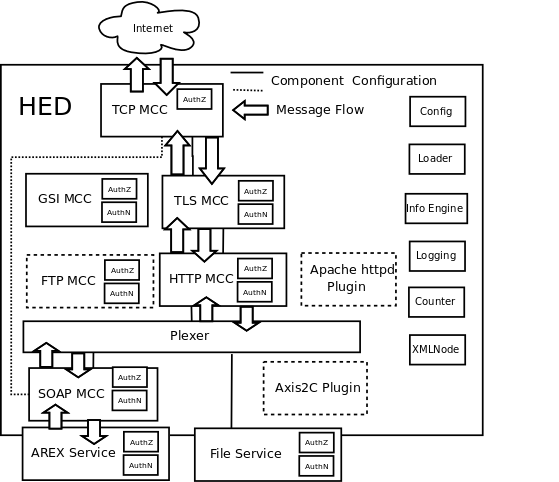
\includegraphics[width=4.0673in,height=3.1047in]{Secpaper-img1.png}
\end{center}
The architecture of the Host Environment Daemon is illustrated as Figure
1. In general, there are a few \ components called MCC (Message Chain
Components) which are in charge of processing different messages for
different protocol levels. For instance, as shown in the example
message flow, HTTP MCC will process secure socket stream from TLS MCC
to generate output HTTP message to SOAP MCC, and also process SOAP
documentation from SOAP MCC to generate HTTP message to TLS MCC. 

Two examples of MCC components configuration in Figure 1 shows MCC are
configurable: real line shows SOAP over HTTPS (HTTP over TLS), while
dotted line shows SOAP directly over TCP. Service administrator can
configure the MCCs according to his requirement, such as the
interoperability requirement with the other part. For instance, the
later configuration is compatible to WSE (Web Services Enhancement for
.NET) {\textquotesingle}s SOAP message mechanism (see
WSE{\textquotesingle}s \textit{SoapSender} and \textit{SoapReceiver}).
Another configuration could be SOAP over HTTPG (HTTP over GSI) which
can be user to interoperate with some service based on HTTPG such as
SRM (Storage Resource Manager) [ref] service. The easily configurable
characteristics shows the flexibility of HED in terms of protocol
supporting.

Because in the current state HED mostly provides modules for building
SOAP based Web Services, it is easy to think that HED is just another
Web Services development framework like Axis, gSOAP, XFire or any other
out of the numerous implementations. Instead, the idea of HED is to
provide framework for gluing functionalities and not a
re-implementation of various standards. Effectively that means if
Apache httpd web server is considered by developers as necessary for
serving as front-end to services there could be plugin code written
which places Apache2 into a chain of other plugins of the HED, the same
for the Apache Axis SOAP implementation, as shown in Figure 1.

Even though the external solutions like Axis and Apache httpd can be
used for protocol supporting, \ two protocols are completely developed
in HED to support HTTP and SOAP in order to make the solution
lightweight and needed an implementation of those supported protocols
that is both simple and lightweight. However external solutions are
used whenever is appropriate - as in the case of TLS (openssl is used),
GridFTP (GridFTP API is used), LDAP and some other cases, this
principle applies to Axis and Apache httpd if we used the API from
those solution to implement the plugins for supporting SOAP and HTTP
protocol. 

HED contains a framework for implementing and enforcing authentication
and authorization. Each Message Chain Component (MCC) or service has a
common interface for implementing various authentication and
authorization functionality. This functionality is implemented by using
pluggable and configurable components (plug-ins) called
\textit{SecHandler}. The \textit{SecHandler} components are C++ classes
and provide method for processing messages traveling through Message
Chains of the HED. Each MCC or Service \ usually implement two queues
of SecHandlers -- one for incoming messages and one for outgoing called
{\textquotedblleft}incoming{\textquotedblright} and
{\textquotedblleft}outgoing{\textquotedblright} respectively. All
\textit{SecHandler} components attached to the queue are executed
sequentially. If any of them fails, message processing fails as well.
In figure 1, the {\textquotedblleft}AuthZ{\textquotedblright} and
{\textquotedblleft}AuthN{\textquotedblright} sub-module inside MCCs and
Services are examples of \textit{SecHandler}.

As explained above, HED is supposed to act as a service holder, but on
the client side, from implementation perspective, there is similar
architecture implemented for processing messages from different
protocols and handling security functionality, also there is a specific
application programming interface (API) for developers to easily write
Web Service client code to service.


\bigskip

{\centering
3. Cross-domain authentication and Single Sign-On
\par}

For cross domain authentication, our work comprises the following five
major aspects:

\liststyleLiii
\begin{itemize}
\item \textit{Integration of community authentication} -{}-{}- to
utilize the standardized community authentication from Shibboleth
Identity Provider software when users authenticate against Grid
services.
\item \textit{Short lived credential service} \ {}-{}-{}- to issue the
short lived X.509 certificate for user by using the community
authentication, in order to interoperate with services that depends on
PKI based mutual authentication.
\end{itemize}

\bigskip

\ \ 3.1 Community based authentication for Grid by utilizing Shibboleth
Identity Provider

AAI (Authentication and authorization Infrastructure) is a solution for
the authentication and authorization for inter-organization resource
sharing, such as electronic resource sharing between libraries, etc.
AAI implicitly applies to community/institutional/organization based
authentication where users are from different home communities but need
to get resources from other communities by using some federation
mechanism. Unlike the X.509 based authentication solution in current
grid systems, AAI does not require user to provide X.509 certificate,
instead, it can support different types of authentication, such as
username/password based authentication, IP address based
authentication, etc. There are a few implementations about AAI, among
which Shibboleth [ref] is one implementation which has been widely
deployed.

Shibboleth provides cross-domain single sign-on and attribute-based
authorization while preserving user privacy. Shibboleth is based on the
OASIS Security Assertion Markup Language (SAML), especially the \ new
version of Shibboleth supports SAML 2.0 specification. For
authentication, the main SAML profile that Shibboleth implements is the
SAML2.0 web browser SSO profile, which \ define two functional
components, an Identity Provider and a Service Provider. The Identity
Provider (IdP) is responsible for creating, maintaining, and managing
user identity, while the Service Provider (SP) is responsible for
controlling access to services and resources by using the SAML
assertion produced and issued by IdP upon request. In order to discover
which home community does a user from, Shibboleth specifies an optional
third component called {\textquotedblleft}Where Are You
From?{\textquotedblright} (WAYF) service to aid in the process of IdP
discovery, and this IdP discovery process is also standardized and
\ defined in SAML 2.0 specification and called as
{\textquotedblleft}Identity Profile Discovery
Profile{\textquotedblright}.

We utilized the SAML2.0 web browser SSO profile for the authentication
in ARC middleware. But since the SSO profile is initially supposed to
protect web applications and provide authentication for web users, we
implemented some external code on the client and service side to
integrate SSO profile. On the client side, apart from the WS-Client API
for writing Web Service client, we implemented the user agent
functionality of web browser in order to mimic the behavior of web
browser{\textquotesingle}s user agent, such as http redirection, cookie
processing, etc. In fact, the implementation of user agent is also
based on the client interface of ARC, specifically, the https client
interface, since the client interface of ARC can support different
protocols which are incarnated by different message chain component
(MCC). Hence client developers who would use SAML2.0 SSO profile should
call the user agent interface and then the WS-Client interface. On the
service side, we implemented the Service Provider functionality (based
on the HTTP MCC configured together with TLS MCC) which is called SP
Service. For Identity Provider, the Shibboleth IdP implementation is
used.

Figure 2 shows the process of SAML2.0 SSO integrated in ARC client and
service.



\begin{center}
\includegraphics[width=3.398in,height=2.1555in]{Secpaper-img2.png}
\end{center}

\bigskip

{\centering
Figure 2. SAML2.0 SSO profile in ARC
\par}

The steps shows in Figure 2 are described as follows:

\liststyleLv
\begin{enumerate}
\item The client use the user agent interface to launches a http request
including the IdP name (to which the user belongs) to the service side.
The host-name and port of destination URL is the same as that of the
real service, the last part of the destination URL is
{\textquotedblleft}saml2sp{\textquotedblright} which is specific for
pointing to the Service Provider. Note that we use Identity Provider
(IdP) name here to simplify the IdP discovery process, because we
suppose that user who would access the service should better know where
is he from initially.
\item The SP Service (Service Provider) searches the metadata (we use
the same metadata with the same format defined in Shibboleth) and gets
the location of the single sign-on service (hosted in IdP) and also the
location of assertion consuming service (hosted in this SP itself) in
order to compose the SAML {\textless}AuthnRequest{\textgreater}
message. Then SP Service issues this
{\textless}AuthnRequest{\textgreater} message by using its own X.509
certificate (Note in the SAML SSO profile, certificate is still needed
by IdP and SP) and sends back to user agent.
\item User agent sends the {\textless}AuthnRequest{\textgreater} message
to Identity Provider.
\item Identity Provider requires an act of authentication. The
authentication mechanism is outside of the SAML2.0 SSO profile. The
shibboleth IdP implementation will choose some login handler for
authentication. The current user agent implementation is compatible to
the Username/Password login handler of Shibboleth IdP. Through the http
protocol, user agent will feed IdP with the username/password which has
been given by the caller of user agent interface.
\item Once the authentication has been succeeded, the IdP issues a SAML
response including an encrypted (encrypted by destination
SP{\textquotesingle}s public key) SAML assertion, and then this SAML
response will be delivered by the user agent to the Service Provider. 
\item The SP Service verifies and checks the SAML response, and decrypts
and stores the SAML assertion into session/connection context. The SAML
assertion actually includes the {\textless}AuthnStatement{\textgreater}
and {\textless}AttributeStatement{\textgreater}.
\item The WS-Client launches the real Grid/Web Service request via the
same connection as the one which is used by user agent to contacts SP
Service.
\item The Grid/Web Service checks the
{\textless}AuthnStatement{\textgreater} from the session context to see
if the session is still valid through the \textit{SecHandler} called
{\textquotedblleft}SAML SecHandler{\textquotedblright}. And if valid,
service handles the real service processing and returns the response to
WS client. Note that service requires WS client is from the same
connection as the one on which user agent contact SP service in order
to guarantee that the validity of SSO profile result effects the real
client/service interaction.
\end{enumerate}
The SP service and real functional service(s) are hosted by the same
container, and they use the same X.509 credential. The client side
authentication is switched off, so that client doesn{\textquotesingle}t
need to use any X.509 credential. Only the trusted certificates (CA
certificate for SP and IdP) need to be configured for client side so
that SP and IdP can authenticate themselves to the client. As required
by SAML2.0 profile, the SP and IdP should have trust relationship to
each other.

Since the Shibboleth implementation of SAML is standard-compliant and
widely deployed, the solution implemented in ARC can easily
interoperate with other SAML implementations with minimum changes, and
more importantly, this solution can succeed to utilize the widely
deployed SAML implementation for authentication in grid systems by
avoiding the usage of X.509 certificate.

Moreover, even though the implementation is based on ARC middlerware,
the idea can be adopted by other grid middlewares if they can only
require server SSL authentication instead of mutual SSL authentication.


\bigskip

\ \ 3.2 Short lived credential service

However, the \ \ Based on the solution described in Section 3.1, 


\bigskip



\begin{center}
\includegraphics[width=4.2134in,height=3.8972in]{Secpaper-img3.png}
\end{center}
{\centering
Figure 3. Short lived credential service
\par}


\bigskip

how to compose the DN


\bigskip

command line


\bigskip


\bigskip


\bigskip

\ \ 3.3 Certificate delegation service


\bigskip


\bigskip

\ \ 3.4 From transport level security to message level security: X.509
Token and SAML Token


\bigskip


\bigskip

\ \ 3.5 Delegation between WS-Security tokens


\bigskip


\bigskip

{\centering
4. Standardized Attribute-based authorization 
\par}


\bigskip

4.1 SAML Attribute Query profile


\bigskip

4.2 Client to VOMS Attribute authority Service


\bigskip

4.3 Attribute parsing and Policy decision point


\bigskip


\bigskip


\bigskip

{\centering
5. Related work
\par}

VOMS AA Service

Shibboleth

GridShib

gLite Delegation Service?

SWITCH SLCS Service

the CCGrid 06 paper: Shibboleth-Protected privilege management
infrastructure


\bigskip


\bigskip

{\centering
6. Conclusion and Future work
\par}


\bigskip


\bigskip

Reference:

Foster I, Kesselman C, Tuecke S. The anatomy of the Grid: Enabling
scalable virtual organizations. International Journal of Supercomputer
Applications 2001; 15(3):200--222. 


\bigskip

The Shibboleth Project.
\href{http://shibboleth.internet2.edu/}{Http://shibboleth.internet2.edu/}


\bigskip
\end{document}
